\section{Quantitative equilibrium paths}
\label{sec:rewrite-quantitative}

\subsection{Parameters and initial conditions}
\label{subsec:rewrite-calibration}

I compare four economies with the same parameters and predetermined initial
stocks, varying only $\sigma$. Table~\ref{tab:rewrite-parameters} retains the
macroeconomic benchmarks used in the earlier specification. The AI parameters
are illustrative, not estimated. All four economies have autonomous research
and a positive AI weight; the no-AI economy in Remark~\ref{rem:rewrite-no-ai}
is not one of these four scenarios.

\begin{table}[H]
\centering
\caption{Parameters and scenario choices}
\label{tab:rewrite-parameters}
\small
\setlength{\tabcolsep}{4pt}
\renewcommand{\arraystretch}{1.10}
\begin{tabular}{P{0.10\textwidth}P{0.17\textwidth}P{0.27\textwidth}P{0.35\textwidth}}
\toprule
Parameter & Value & Interpretation & Source or rationale\\
\midrule
$\alpha$ & 0.33 & Capital elasticity & Standard one-third macro benchmark\\
$\delta$ & 0.05 & Annual capital depreciation & Annual benchmark; PWT comparison \citep{pwt110}\\
$\rho$ & 0.04 & Annual household discount rate & Preference calibration\\
$n$ & 0.003 & Annual population growth & Constant-rate approximation to the UN 2024--2100 world projection \citep{unwpp2024}\\
$\gamma$ & 0.01 & Annual growth of labor-augmenting technology & Illustrative long-run trend; see \citet{oecdlongrun2025}\\
$\omega_X$ & 0.20 & Weight on effective AI production services & Scenario choice, not an observed industry share\\
$\omega_L$ & 0.80 & Weight on effective labor & $1-\omega_X$\\
$\eta$ & 0.20 & Research exponent & Assumptions~\ref{ass:rewrite-research-curvature} and~\ref{ass:rewrite-research-concavity}\\
$\chi$ & 1.4378 & Research productivity & Calibrated transition-speed parameter\\
$\sigma$ & 0.90; 1; 1.10; 1.50 & AI--labor substitution & Four scenarios spanning the analytical regimes\\
$\overline B$ & $1.10\,\overline B_c(1.50)$ $\simeq170.124$ & Common AI-efficiency frontier & Ten percent above the threshold for $\sigma=1.50$\\
\bottomrule
\end{tabular}
\end{table}

The constant $n$ extrapolates a finite-period demographic approximation; it
is not a claim that the UN projects constant population growth forever.
The OECD benchmark for $\gamma$ concerns measured labor-productivity growth,
not $A$ directly. I use it only as an approximate guide to the magnitude of
long-run labor-augmenting technological progress.
The parameter $\chi$ determines research speed relative to the other annual
rates, so it is not merely a free time-unit normalization. I choose
$\chi=1.4378$ so that, in the $\sigma=1.50$ equilibrium, the labor income share
completes half of the distance between its date-zero value and its analytical
limit after 50 model years. This is an illustrative timing normalization, not
an estimate. Different values of $\chi$ produce faster or slower transitions
and require the entire equilibrium path to be solved again. The horizontal
axes below measure model years, not calendar forecasts. Likewise, the OECD's
discussion of AI-investment measurement supports treating $\omega_X$ as a
scenario parameter, but does not identify its value
\citep{oecdaiinvestment2025,oecdproductivity2026}.

The common frontier is below $\overline B_c(1.10)\simeq60.4$ million but above
$\overline B_c(1.50)\simeq154.658$. Thus $\sigma=1.10$ retains a positive
long-run labor share, whereas $\sigma=1.50$ enters the AI-dominated regime.
Changing the frontier separately across scenarios would confound this
comparison of elasticities.

I set
\begin{equation}
 A_0=N_0=1,\qquad K_0=4,\qquad B_0=0.10\overline B\simeq17.0124.
 \label{eq:rewrite-simulation-initial-stocks}
\end{equation}
These common initial stocks place the economy closer to the capped
$\sigma=1$ terminal regime than the earlier uncapped reference: initial AI
efficiency is 10 percent of its frontier and initial capital per unit of
effective labor is about 44 percent of its terminal $\sigma=1$ value. They are
not a balanced-growth state of the capped economy. An exact constant-efficiency reference at
$B_0=\overline B$ would eliminate further improvements in AI efficiency and would
lie outside the interior problem studied here. In each capped economy, the
BVP selects $C_0$ and $q_0$ anew; neither jump variable is fixed at its
uncapped reference value.

\subsection{Numerical method and equilibrium admission}
\label{subsec:rewrite-method}

I retain the four-dimensional boundary-value architecture: two initial stock
conditions and two terminal conditions selecting the stable equilibrium
continuation. The appropriate finite-frontier regime from
Section~\ref{sec:rewrite-regimes}, not the uncapped unit-elastic BGP, determines
the terminal conditions. Appendix~\ref{app:rewrite-algorithm} documents the
continuation, equation reconstruction, and numerical checks.

In economic terms, the algorithm takes $K_0$ and $B_0$ as given and selects
the initial consumption and shadow value that place the economy on the stable
equilibrium path. It first constructs that path near the analytically
characterized terminal regime and then moves it gradually to the prescribed
initial stocks. Solving the boundary-value problem is only the construction
step; the separate admission tests determine whether the resulting candidate
is reported as an equilibrium.

A converged BVP is not sufficient for admission. I also check feasibility,
independently reconstructed dynamic residuals, stability to longer horizons
and tighter tolerances, both transversality conditions, and sufficient global
developer optimality. The first three scenarios satisfy the global concavity
test. For $\sigma=1.50$, that stronger test fails at low counterfactual
AI-efficiency levels, but the Hamiltonian support test in
Proposition~\ref{prop:rewrite-hamiltonian-support} passes. Its analytical
long-run bound is given in \eqref{eq:rewrite-support-terminal-bound}.

\subsection{Growth, prices, and the distribution of output}
\label{subsec:rewrite-distribution}

Figures~\ref{fig:rewrite-accumulation-growth}--\ref{fig:rewrite-ai-distribution}
present the transition in three steps: quantities and accumulation, prices and
returns, and the distribution of output. Each panel includes the same four
admitted trajectories. The three labor-bottleneck paths consequently appear
close to one another in several panels. This compression reflects their common
long-run regime; exact initial and limiting values of the central outcomes are
reported in Table~\ref{tab:rewrite-central-path-values}.

\Needspace{10\baselineskip}
The relative growth of effective AI production services is central to reading
the figures. Rearranging \eqref{eq:rewrite-sx} gives
\begin{equation}
 \frac{s_X}{1-s_X}
 =\frac{\omega_X}{\omega_L}
 \left(\frac{X}{AL}\right)^{(\sigma-1)/\sigma}.
 \label{eq:rewrite-transition-share-odds}
\end{equation}
Differentiating this expression yields
\begin{equation}
 \frac{d}{dt}\log\!\left(\frac{s_X}{1-s_X}\right)
 =\frac{\sigma-1}{\sigma}\left[g_X-(n+\gamma)\right].
 \label{eq:rewrite-transition-share-growth}
\end{equation}
Thus the growth of $X/(AL)$ determines the direction and speed at which the
AI share changes, conditional on $\sigma$.

Figure~\ref{fig:rewrite-accumulation-growth} first reports the growth rates of
output, effective AI production services, and capital per unit of effective
labor. These are $g_Y-(n+\gamma)$, $g_X-(n+\gamma)$, and
$g_K-(n+\gamma)$, respectively. Growth rates show when the economy accelerates
without compressing the large level differences that emerge across regimes.

\begin{figure}[H]
 \centering
 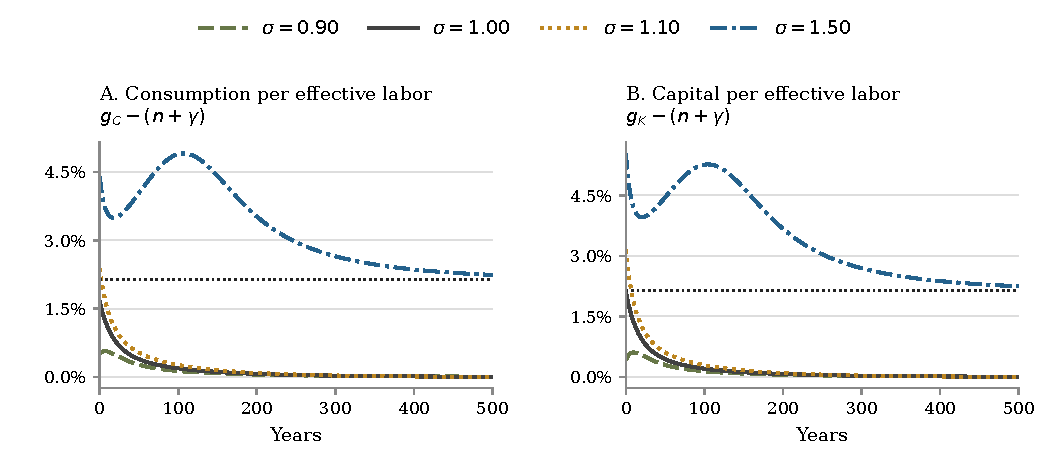
\includegraphics[width=\textwidth]{figures_rewrite/equilibrium_accumulation_growth.pdf}
 \caption{Growth of output, effective AI production services, and capital per
 unit of effective labor. Each panel compares the same four admitted numerical
 equilibrium trajectories over 500 model years. Panels A and C use the same
 linear percentage scale; Panel B uses a separate linear percentage range.
 Thin horizontal dotted lines mark the analytical limits for $\sigma=1.50$.}
 \label{fig:rewrite-accumulation-growth}
\end{figure}

\Needspace{10\baselineskip}
Figure~\ref{fig:rewrite-growth-returns} next reports real-wage growth, the net
interest rate, and the price of effective AI production services. The first
two are rates; $p_X$ is a relative-price level measured in units of the final
good. Equation~\eqref{eq:rewrite-markup} implies
$p_X=1/[B(1-e_X)]$. Because $B$ approaches its finite frontier and $e_X$
approaches a value below one in every terminal regime, $p_X$ converges to a
positive finite level. It falls rather than grows without bound in all four
simulations. I therefore report its level on a logarithmic scale, which keeps
the four positive price paths visible despite their different magnitudes.

\begin{figure}[H]
 \centering
 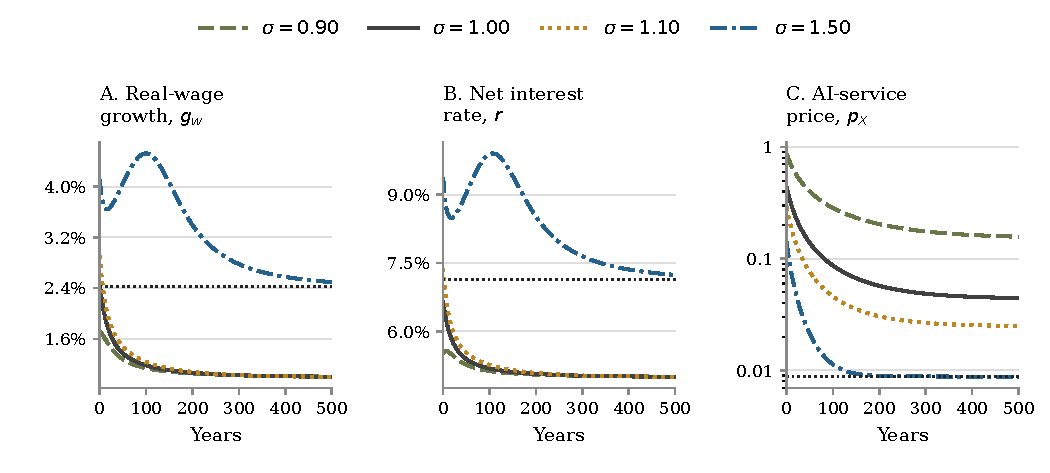
\includegraphics[width=\textwidth]{figures_rewrite/equilibrium_growth_returns.pdf}
 \caption{Wages, returns, and the AI-service price. Each panel compares the same
 four admitted numerical equilibrium trajectories over 500 model years.
 Real-wage growth and the net interest rate use linear percentage scales.
 The level of $p_X$ uses a logarithmic scale. Thin horizontal dotted lines mark
 the analytical limits for $\sigma=1.50$.}
 \label{fig:rewrite-growth-returns}
\end{figure}

Finally, Figure~\ref{fig:rewrite-ai-distribution} reports labor income and the
three uses of AI-industry revenue as shares of final output. Combining final-good
zero profit with $\Pi=p_XX-U-M$ gives
\begin{equation}
 \frac{wL}{Y}+\frac{\Pi}{Y}+\frac{U}{Y}+\frac{M}{Y}=1-\alpha.
 \label{eq:rewrite-noncapital-distribution}
\end{equation}
The four panels therefore exhaust the noncapital share of output. Gross capital
income, $(r+\delta)K/Y=\alpha$, is constant and accounts for the remainder.

\begin{figure}[H]
 \centering
 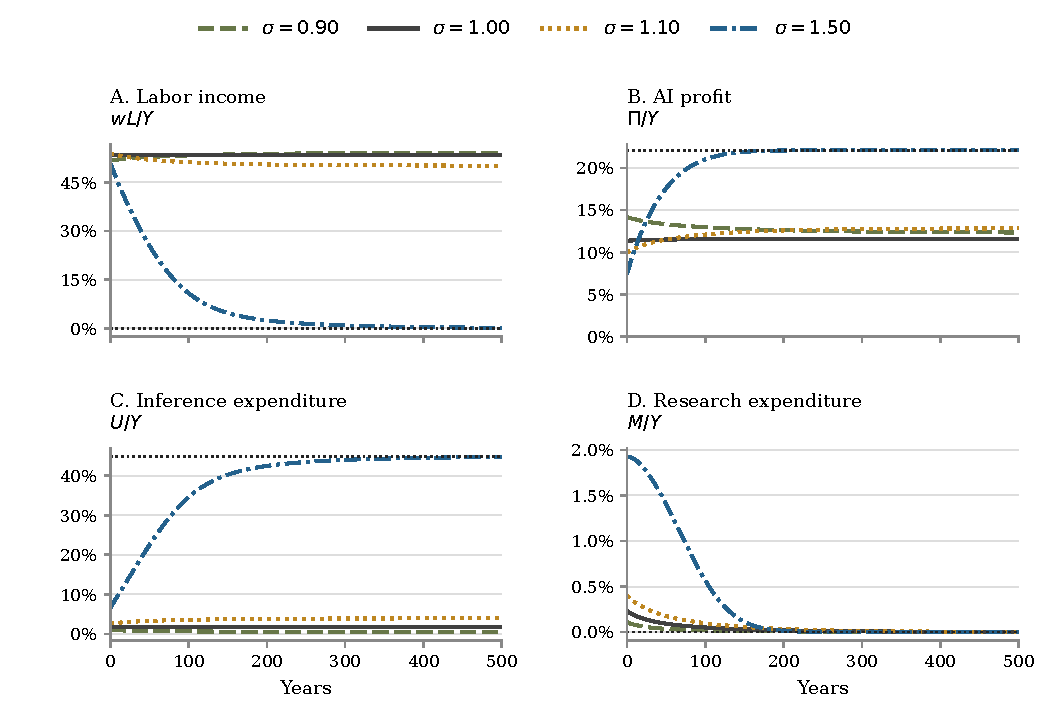
\includegraphics[width=\textwidth]{figures_rewrite/equilibrium_ai_distribution.pdf}
 \caption{Distribution of the noncapital share of output. The panels report
 labor income, AI profit, inference expenditure, and research expenditure,
 each divided by final output. Together they sum to $1-\alpha$; the omitted
 gross capital-income share is the constant $\alpha$. Each panel compares the
 same four admitted numerical equilibrium trajectories over 500 model years
 and uses a linear percentage scale. Thin horizontal dotted lines mark the
 analytical limits for $\sigma=1.50$.}
 \label{fig:rewrite-ai-distribution}
\end{figure}

\begin{table}[H]
\centering
\caption{Initial and long-run values of the central outcomes}
\label{tab:rewrite-central-path-values}
\small
\setlength{\tabcolsep}{5pt}
\begin{tabular}{ccrrrrr}
\toprule
$\sigma$ & Date & $g_Y-n$ & $g_w$ & $r$ & $wL/Y$ & $p_XX/Y$\\
\midrule
0.90 & $0$      & 1.629 & 1.711 & 5.508 & 51.7 & 15.3\\
     & $\infty$ & 1.000 & 1.000 & 5.000 & 54.2 & 12.8\\
1.00 & $0$      & 2.458 & 2.458 & 6.646 & 53.6 & 13.4\\
     & $\infty$ & 1.000 & 1.000 & 5.000 & 53.6 & 13.4\\
1.10 & $0$      & 3.046 & 2.909 & 7.380 & 54.0 & 13.0\\
     & $\infty$ & 1.000 & 1.000 & 5.000 & 50.2 & 16.8\\
1.50 & $0$      & 5.390 & 4.115 & 9.385 & 51.0 & 16.0\\
     & $\infty$ & 3.135 & 2.423 & 7.135 & 0.0 & 67.0\\
\bottomrule
\end{tabular}

\vspace{2pt}
\parbox{0.94\textwidth}{\footnotesize\emph{Note:} All entries are percentages.
Date-zero entries come from the numerical equilibrium paths. Infinite-date
entries are the analytical limits characterized in Section~\ref{sec:rewrite-regimes}.}
\end{table}

The first three scenarios approach per-person growth of $1\%$ and a net
interest rate of $5\%$. For $\sigma=1.50$, their analytical limits are
$3.135\%$ and $7.135\%$, respectively. Real wages then grow asymptotically
at $2.423\%$. Thus output per person grows $0.712$ percentage points faster
than the real wage. By Proposition~\ref{prop:rewrite-output-wage-wedge}, this
implies an asymptotic decline of $0.712\%$ per year in the log labor income
share. The central distributional result is therefore not that real wages decline:
workers become richer in absolute terms while their claim on total output
vanishes. AI revenue meanwhile approaches $67\%$ of output. These limiting
rates describe the equilibrium continuations; they are not imposed as
constant rates during the transition.

The AI-dominated path also displays signals before labor's income share has
fallen sharply. At date zero, $X/(AL)$ grows at $16.051\%$ and the net interest
rate is $9.385\%$, well above the $5\%$ labor-bottleneck benchmark, while labor
still receives $51.0\%$ of output. Moreover, because $L=N$, the accounting
identity
\begin{equation}
 \frac{d}{dt}\log\!\left(\frac{wL}{Y}\right)
 =g_w-(g_Y-n)
 \label{eq:rewrite-transition-labor-share-identity}
\end{equation}
holds at every date. The gap between output-per-person and real-wage growth
therefore does not merely predict a later distributional change: a positive
gap is exactly the contemporaneous rate at which the log labor income share
declines, and a widening gap means that decline is accelerating.

Equations~\eqref{eq:rewrite-transition-share-odds} and
\eqref{eq:rewrite-transition-share-growth} provide the structural explanation
for the speed of the transition. A value $\sigma>1$ makes the AI share rise
with $X/(AL)$, but it does not make
AI immediately replace labor. When $\sigma$ is close to one, the exponent
$(\sigma-1)/\sigma$ is small and the share responds slowly even to large
increases in relative AI services. At $\sigma=1.50$, for example, the
exponent is $1/3$: increasing the odds $s_X/(1-s_X)$ by a factor of ten
requires a thousand-fold increase in $X/(AL)$. For elasticities closer to
one, the required increase is larger still, conditional on the frontier
being high enough to support the AI-dominated regime.

The economy must also accumulate the inputs that produce this change.
Neither $K$ nor $B$ can jump. Expanding $X$ requires inference compute
$U=X/B$, while improving $B$ requires research compute $M$; both uses compete
with consumption and physical investment for current output. Moreover,
$\eta=0.20$ implies strong diminishing returns to a contemporaneous increase
in research compute. As $B$ rises, however, it reduces the compute required
to supply a unit of $X$ and makes subsequent research compute more productive.
The feedback therefore strengthens gradually. Near the finite frontier,
$\psi(B)$ slows further efficiency improvement. The eventual acceleration in
the AI-dominated equilibrium is consequently not an explosion of $B$: it is
sustained by the expansion of capital and effective AI production services
after labor ceases to be the binding input.

The date of takeoff is not a structural prediction of the model. Equation
\eqref{eq:rewrite-transition-share-odds} implies an earlier transition when
$\sigma$ is farther above one or when $X$ grows faster relative to $AL$.
Within the model, greater research productivity $\chi$, a higher initial
$B_0$, or a larger AI weight $\omega_X$ can advance the transition through
different channels. Faster capital accumulation or slower growth of effective
labor can also allow $X/(AL)$ to rise sooner. These changes are not
interchangeable: $\sigma$ and $\omega_X$ alter the production technology,
$B_0$ changes the initial economy, and $\chi$ changes the research clock. The
effects of changing $\eta$ or $\overline B$ on the takeoff date do not have an
unambiguous general-equilibrium sign because they also change research
incentives and the terminal equilibrium. These comparative mechanisms indicate
how the transition may move, but do not identify a date without recalculating
the equilibrium path.

The $\sigma=1.50$ path displays this mechanism under the calibrated research
speed. The labor share completes 10 percent of its decline after 8.3 model
years, half after 50 years, and 90 percent after 145.2 years. At year 50,
output per person grows at $5.616\%$, the real wage at $4.050\%$, and labor
receives $25.5\%$ of output. At year 100, the corresponding growth rates are
$6.290\%$ and $4.522\%$, while labor's share has fallen to $10.9\%$. By year
500, output-per-person growth is $3.239\%$, real-wage growth is $2.494\%$,
and labor's share is $0.19\%$; all three are close to their analytical limits.
The non-monotone growth response reflects the costly initial research surge,
the subsequent acceleration in effective AI services, and eventual convergence
as $B$ approaches its frontier. These dates illustrate an equilibrium under
one research-speed calibration. They are not estimates of when an actual AI
transition will occur.

Substitution alone does not produce this outcome. With the same frontier
and $\sigma=1.10$, the labor share instead approaches $50.2\%$, compared
with $53.6\%$ at $\sigma=1$ and $54.2\%$ at $\sigma=0.90$.
The frontier's position relative to the elasticity-specific threshold is
essential to interpreting the comparison.

\subsection{Near-terminal labor-bottleneck paths}
\label{subsec:rewrite-near-terminal}

The initially high and declining growth rates of the three labor-bottleneck
paths in the main comparison are not their long-run prediction. They partly
reflect the distance between the common initial stocks in
\eqref{eq:rewrite-simulation-initial-stocks} and each economy's terminal
allocation. To isolate terminal behavior, I solve an additional exercise only
for $\sigma\in\{0.90,1,1.10\}$. I set
\begin{equation}
 \frac{B_0}{\overline B}=0.99,
 \qquad
 \frac{K_0}{A_0N_0}=
 \left.\frac{K}{AN}\right|_{\text{terminal}}
 =\begin{cases}
  6.5571,&\sigma=0.90,\\
  9.0990,&\sigma=1,\\
  12.2652,&\sigma=1.10.
 \end{cases}
 \label{eq:rewrite-near-terminal-stocks}
\end{equation}
Consumption and the developer's shadow value are again selected by the BVP
for each path. Because $B_0<\overline B$ and research remains positive, these
are not exact steady states at a finite date. They are equilibrium paths that
begin near their respective terminal regimes. Moreover, because the initial
capital ratio varies with $\sigma$, this exercise isolates terminal behavior;
it is not a comparative experiment holding all initial stocks fixed.

\begin{figure}[H]
 \centering
 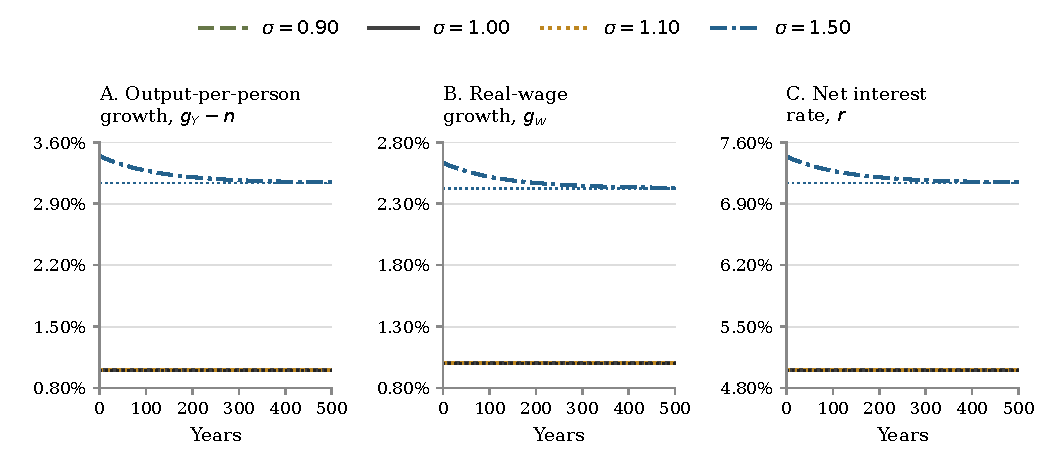
\includegraphics[width=\textwidth]{figures_rewrite/equilibrium_near_terminal_growth_returns.pdf}
 \caption{Near-terminal labor-bottleneck equilibrium paths. The panels report
 output-per-person growth, real-wage growth, and the net interest rate for
 three independently admitted numerical equilibria over 500 model years.
 Thin horizontal dotted lines mark their common analytical limits: $\gamma$
 for both growth rates and $\rho+\gamma$ for the net interest rate. The
 vertical axes cover narrow ranges around those limits.}
 \label{fig:rewrite-near-terminal-growth-returns}
\end{figure}

Figure~\ref{fig:rewrite-near-terminal-growth-returns} removes the large
date-zero movements visible in the main comparison. At date zero,
output-per-person and real-wage growth lie between $0.986\%$ and $0.994\%$,
while the net interest rate lies between $4.977\%$ and $4.990\%$. The three
paths then remain close to, and converge toward, their common analytical
limits of $1\%$, $1\%$, and $5\%$. The exercise therefore confirms that the
high initial growth rates in the main labor-bottleneck paths are transitional
responses to the common starting stocks, rather than properties of the
labor-bottleneck long run.

\subsection{A slower transition}
\label{subsec:rewrite-slow-transition}

The 50-year midpoint in the main comparison is a timing calibration rather
than a prediction. To show how strongly the transition can stretch out, I
recover the earlier calibration with
\begin{equation}
 \chi=0.01,\qquad K_0=2.027733654,\qquad B_0=0.443670932.
 \label{eq:rewrite-slow-transition-design}
\end{equation}
All other parameters, the common frontier, and the four values of $\sigma$
are unchanged. These initial stocks come from the uncapped unit-elastic BGP,
but neither the initial consumption nor the initial shadow value is imported
from it. Both jump variables are solved again for each capped economy. The
exercise changes both research productivity and the initial distance from the
frontier, so it should not be interpreted as a one-parameter estimate of the
effect of $\chi$. Each of the four paths is independently re-solved and passes
the same equilibrium-admission tests as the main comparison.

Figures~\ref{fig:rewrite-slow-accumulation-growth}--
\ref{fig:rewrite-slow-ai-distribution} retain the variables, normalizations,
scenario order, and scale conventions of the main figures. The only
presentational change is the 4,000-year window needed to display the slower
adjustment.

\begin{figure}[H]
 \centering
 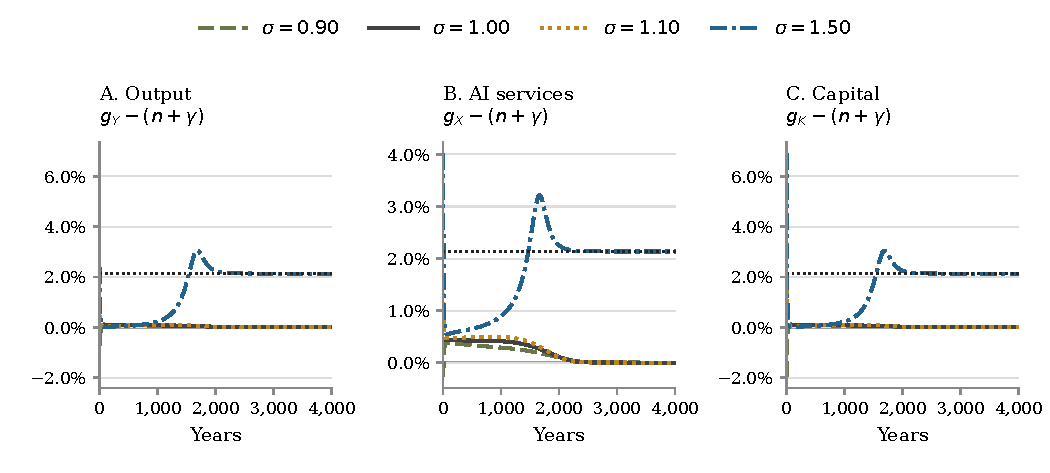
\includegraphics[width=\textwidth]{figures_rewrite/equilibrium_slow_accumulation_growth.pdf}
 \caption{Growth of output, effective AI production services, and capital per
 unit of effective labor under the slower-transition calibration. Each panel
 compares the same four admitted numerical equilibrium trajectories over
 4,000 model years. Panels A and C use the same linear percentage scale;
 Panel B uses a separate linear percentage range. Thin horizontal dotted
 lines mark the analytical limits for $\sigma=1.50$.}
 \label{fig:rewrite-slow-accumulation-growth}
\end{figure}

\begin{figure}[H]
 \centering
 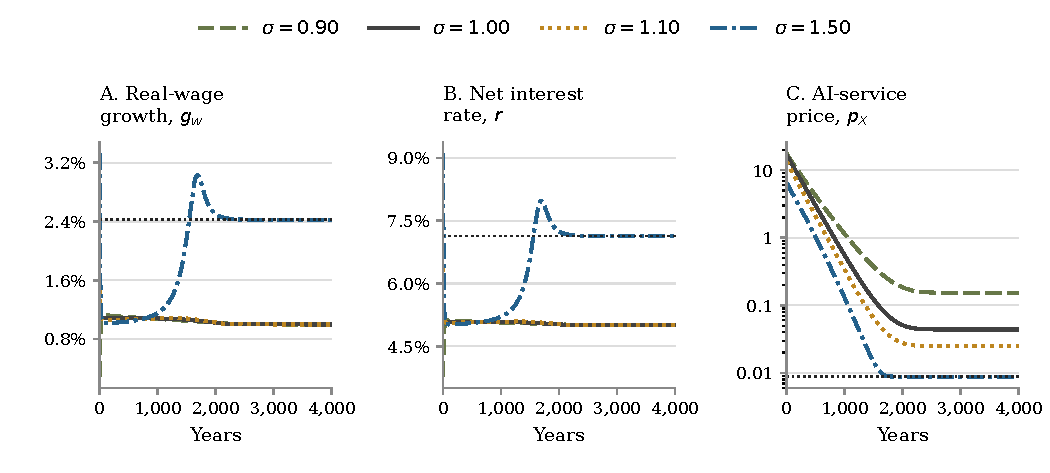
\includegraphics[width=\textwidth]{figures_rewrite/equilibrium_slow_growth_returns.pdf}
 \caption{Wages, returns, and the AI-service price under the slower-transition
 calibration. Each panel compares the same four admitted numerical equilibrium
 trajectories over 4,000 model years. Real-wage growth and the net interest
 rate use linear percentage scales; the level of $p_X$ uses a logarithmic
 scale. Thin horizontal dotted lines mark the analytical limits for
 $\sigma=1.50$.}
 \label{fig:rewrite-slow-growth-returns}
\end{figure}

\begin{figure}[H]
 \centering
 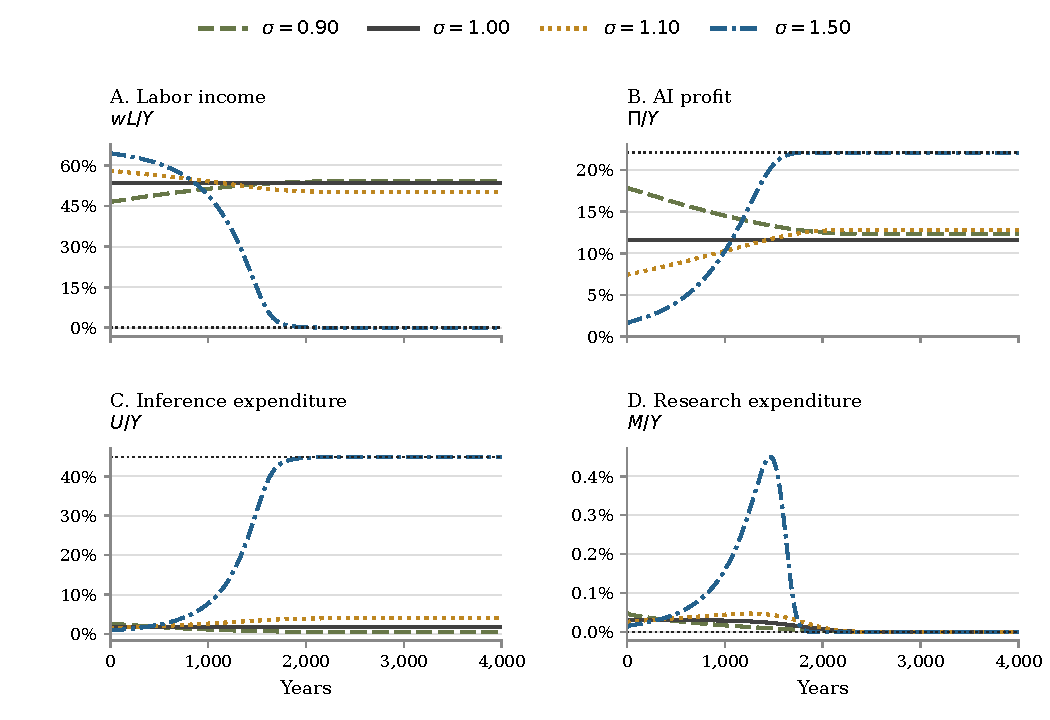
\includegraphics[width=\textwidth]{figures_rewrite/equilibrium_slow_ai_distribution.pdf}
 \caption{Distribution of the noncapital share of output under the
 slower-transition calibration. Labor income, AI profit, inference expenditure,
 and research expenditure are divided by final output and sum to $1-\alpha$.
 The omitted gross capital-income share is the constant $\alpha$. Each panel
 compares the same four admitted numerical equilibrium trajectories over
 4,000 model years. Thin horizontal dotted lines mark the analytical limits
 for $\sigma=1.50$.}
 \label{fig:rewrite-slow-ai-distribution}
\end{figure}

In the slow $\sigma=1.50$ equilibrium, labor's income share completes only
10 percent of its decline after 657 model years, half after 1,295 years, and
90 percent after 1,605 years. At year 500, output per person grows at
$1.062\%$, the real wage at $1.043\%$, and labor still receives $60.5\%$ of
output. By year 1,500, output-per-person growth has risen to $2.797\%$, while
labor's share has fallen to $14.5\%$. The analytical limits are the same as in
the main comparison because $\sigma$ and $\overline B$ are unchanged; what
changes radically is when the economy approaches them. The model can therefore
generate a long interval in which little appears to happen before growth and
the distribution of output change sharply. It does not identify which of the
two timing calibrations is empirically more plausible.

\subsection{Initial financing sensitivity}
\label{subsec:rewrite-technology-revenue}

Moving the common initial stocks closer to the $\sigma=1$ terminal regime
materially reduces the initial financing requirement. In the reported
$\sigma=1.50$ path, research absorbs $12.0\%$ of AI revenue, inference absorbs
$41.4\%$, and the developer distributes the remaining $46.6\%$ as profit.
These quantities equal $1.92\%$, $6.60\%$, and $7.44\%$ of final output,
respectively.

This benign date-zero composition is not invariant to the initial stocks. In
an admitted sensitivity path that begins much farther from the terminal regime,
at $K_0=2.0277$ and $B_0/\overline B=0.26\%$, and recalibrates $\chi$ to preserve
the same 50-year midpoint, research expenditure initially equals $106.0\%$ of
AI revenue and profit is $-40.5\%$ of AI revenue. The household owner then
finances the loss through an equity injection because current research raises
$B$ and the present value of future monopoly rents. The benchmark permits this intertemporal
financing: it imposes neither a borrowing constraint nor a nonnegative-profit
constraint on the developer. Adding such a constraint could delay or restrict
the transition. The contrast therefore identifies initial technological
distance and financing capacity as substantive determinants of the transition,
not as innocuous plotting choices.

In the AI-dominated limit, inference absorbs $67\%$ of AI revenue, research's
revenue share vanishes, and the developer retains $33\%$. Its net distribution
therefore approaches $22.11\%$ of final output. By contrast, at $\sigma=1$
AI revenue is always $13.4\%$ of output and inference absorbs $13.4\%$ of
that revenue. A vanishing research share does not mean that research stops:
the constructed finite-frontier equilibria have a positive limiting level of
research compute, while industry revenue continues to grow.
